% !TeX root = RJwrapper.tex
\title{rentrez: An R package for the NCBI eutils API}
\author{by David J. Winter}

\maketitle

\abstract{
The USA National Center for Biotechnology Information (NCBI) is one of the
world's most important sources of biological information. NCBI databases like
PubMed and GenBank contain millions of records describing bibliographic,
genetic, genomic, and medical data. Here I present \pkg{rentrez}, a package
which provides an R interface to 50 NCBI databases. The package is
well-documented, contains an extensive suite of unit tests and has an active
user base. The programmatic interface to the NCBI provided by \pkg{rentrez}
allows researchers to query databases and download or import particular records
into R sessions for subsequent analysis. The complete nature of the package, 
its extensive test-suite and the fact the package implements the NCBI's
usage policies all make \pkg{rentrez} a powerful aid to developers of new
packages that perform more specific tasks.
}

\section{Introduction}

The USA National Center for Biotechnology Information (NCBI) is one of the world's 
largest and most important sources of biological data. At the time of writing, the NCBI
PubMed database provided information on $27.5$ million journal
articles, including $4.6$ million full text records. The NCBI
Nucleotide Database (including GenBank) had data for $243.3$ million different sequences and dbSNP described $997.3$ 
million different genetic variants. Records from all of these databases can be 
cross-referenced with the $1.3$ million species in the NCBI taxonomy, and PubMed entries can be searched using a 
controlled vocabulary containing $272$ thousand unique terms. 

The NCBI provides access to a total of $50$ databases 
through a web interface, public FTP sites and an API called Entrez Programming
Utilities (EUtils, \citealt{sayers_EUtils}). R packages from the Bioconductor 
project (e.g., \BIOpkg{genomes}, \citealt{genomes}; \BIOpkg{RMassBank}, 
\citealt{RMassBank} and \BIOpkg{MeSHSim}, \citealt{MeSHSim}) or available from 
CRAN (e.g., \CRANpkg{ape}, \citealt{APE}; \CRANpkg{RISmed}, \citealt{RISmed} and
\CRANpkg{pubmed.mineR}, \citealt{miner}) take advantage of the Eutils API to 
perform specific tasks. Two packages, \CRANpkg{rentrez} and \CRANpkg{reutils} 
\citep{reutils}, provide functions that cover the entire API.  Here I describe 
\pkg{rentrez}, a package which provides users with a simple and consistent 
interface to EUtils. This paper discusses the design of the package, illustrates 
its use in biological research and demonstrates how the provided functions can 
aid the development of other packages designed to meet more specific goals.

\section{The EUtils API and \pkg{rentrez} }

The EUtils API provides endpoints for searching each of the databases it covers, 
finding cross-references among records in those databases and fetching 
particular records (in complete or summary form). The design of \pkg{rentrez} 
mirrors that of EUtils, with each of these endpoints represented by a core
function that has arguments named to match those used in the API documentation
(Table \ref{tab:core-ends}). The most important arguments to each R function are
documented, and the help pages associated with these functions contain a reference 
to the relevant section of the EUtils documentation.

\begin{table}[]
\centering
\caption{Core EUtils endpoints and their \pkg{rentrez} counterparts}
\label{tab:core-ends}
\begin{tabular}{llll}
\hline
NCBI endpoint & Purpose                                         & Core function            \\ \hline
esearch       & Locate records matching search criteria.        & \texttt{entrez\_search}  \\
elink         & Discover cross-linked records.                  & \texttt{entrez\_link}    \\ 
esummary      & Fetch summary data on a set of records.         & \texttt{entrez\_summary} \\ 
efetch        & Fetch complete records in a variety of formats. & \texttt{entrez\_fetch}   \\ \hline
\end{tabular}
\end{table}


Typically, a user will begin by using \code{entrez\_search} to discover unique
identifiers for database records matching particular criteria. EUtils allows
users to search against particular terms in each database (the terms available
for a given database can be retrieved with the function
\code{entrez\_db\_searchable}), and to combine queries with boolean operators. 
For example, the following call finds scientific papers that were published in 2017 
and contain the phrase `R Package' in their title.

\begin{example}
pubmed_search <- entrez_search(db="pubmed", 
                               term="(R package[TITL]) AND 2017[PDAT]", 
                               use_history=TRUE)
pubmed_search

#> Entrez search result with 62 hits (object contains 20 IDs and a web_history object)
#>  Search term (as translated):  R package[TITL] AND 2017[PDAT]
\end{example}

The object returned by \code{entrez\_search} can contain identifiers for records that
match the given search term or a \code{web\_history} object that serves as a reference 
to a set of identifiers stored on the NCBI's servers. Identifiers or
\code{web\_history} objects can be passed to the other core functions to retrieve
information about the records they represent. For example, a call to
\code{entrez\_summary} returns information about each paper identified in the search
above.


\begin{example}
pkg_paper_summs <- entrez_summary(db="pubmed", web_history=pubmed_search$web_history)
pkg_paper_summs

#> List of  62 esummary records. First record:
#> 
#>  $`28759592`
#> esummary result with 42 items:
#>  [1] uid               pubdate           epubdate         
#>  [4] source            authors           lastauthor       
#>  [7] title             sorttitle         volume           
#> [10] issue             pages             lang             
#> [13] nlmuniqueid       issn              essn             
#> [16] pubtype           recordstatus      pubstatus        
#> [19] articleids        history           references       
#> [22] attributes        pmcrefcount       fulljournalname  
#> [25] elocationid       doctype           srccontriblist   
#> [28] booktitle         medium            edition          
#> [31] publisherlocation publishername     srcdate          
#> [34] reportnumber      availablefromurl  locationlabel    
#> [37] doccontriblist    docdate           bookname         
#> [40] chapter           sortpubdate       sortfirstauthor
\end{example}

In addition to matching each of the EUtils endpoints, \pkg{rentrez} provides
utility functions that facilitate common workflows. For example, the
function \code{extract\_from\_summary} allows users to extract some subset of
the items contained in each of a set of summary records. In this case, the names of 
the  journals that these papers appeared in can be retrieved. The  resulting 
character vector can then be used to identify the PubMed-indexed journals that 
have published the most papers describing R packages this year.

\begin{example}
journals <- extract_from_esummary(pkg_paper_summs, "fulljournalname")
journals_by_R_pkgs <- sort(table(journals), decreasing = TRUE)
head(journals_by_R_pkgs,3)

#> journals
#> Bioinformatics (Oxford, England)               BMC bioinformatics 
#>                               16                                9 
#>      Molecular ecology resources 
#>                                9
\end{example}

\section{Demonstration: retrieving unique transcripts for a given gene}

Records in the NCBI's various databases are heavily cross-referenced, allowing
users to identify and download data related to particular papers, organisms or 
genes. By providing a programmatic interface to these records \pkg{rentrez}
allows R users to develop reproducible workflows that either download particular
datasets for further analysis or load them into an R session. Here I demonstrate
such a workflow, downloading DNA sequences corresponding to unique
mRNA transcripts of a particular gene in a particular species.

Our aim is to retrieve the sequence of mRNA transcripts associated with the gene 
that encodes Amyloid Beta Precursor Protein in humans. This gene is identified 
by the gene symbol \footnote{\url{http://www.genenames.org/}} \samp{APP}. The 
NCBI database dealing with genetic loci (rather than particular sequences) is 
called `Gene', so the first step to recovering the sequence data is discovering 
the unique identifier associated with APP in this database. This can be 
achieved with \code{entrez\_search}, using the gene symbol and species in the 
search term.

\begin{example}
app_gene <- entrez_search(db="gene", term="(Homo sapiens[ORGN]) AND APP[GENE]")
app_gene

#> Entrez search result with 1 hits (object contains 1 IDs and no web_history object)
#>  Search term (as translated):  "Homo sapiens"[Organism] AND APP[GENE]
\end{example}

We now have a unique identifier for APP in the Gene database. In order to download 
sequences for this gene we need to find records from the NCBI Nucleotide database 
that are associated with the Gene record. The function \code{entrez\_link} can be 
used to find cross-referenced records. In this case, a single call to 
\code{entrez\_link} can identify human APP sequences in the nucleotide database in 
general and in a number of restrictive subsets of that database.

\begin{example}
nuc_links <- entrez_link(dbfrom="gene", id=app_gene$ids, db="nuccore")
nuc_links$links

#> elink result with information from 5 databases:
#> [1] gene_nuccore            gene_nuccore_mgc        gene_nuccore_pos       
#> [4] gene_nuccore_refseqgene gene_nuccore_refseqrna
\end{example}

The RefSeq RNA subset on the Nucleotide database contains a curated set of
mRNA transcripts for different genes. Thus the unique identifiers contained in 
the \code{gene\_nuccore\_refseqrna} element correspond to the sequences we wish 
to download.The function \code{entrez\_fetch} allows users to retrieve complete 
records in a variety of formats. Here the sequences are retrieved in the 
standard \samp{fasta} format, and  returned as a character vector with a single 
element.

\begin{example}
raw_recs <- entrez_fetch(db="nuccore", 
                         id=nuc_links$links$gene_nuccore_refseqrna, 
                         rettype="fasta")                         
cat(substr(raw_recs, 1,303), "...")

#> >NM_001136131.2 Homo sapiens amyloid beta precursor protein (APP) ...
#> GTCGGATGATTCAAGCTCACGGGGACGAGCAGGAGCGCTCTCGACTTTTCTAGAGCCTCAGCGTCCTAGG
#> ACTCACCTTTCCCTGATCCTGCACCGTCCCTCTCCTGGCCCCAGACTCTCCCTCCCACTGTTCACGAAGC
#> CCAGGTACCCACTGATGGTAATGCTGGCCTGCTGGCTGAACCCCAGATTGCCATGTTCTGTGGCAGA...
\end{example}

Sequences retrieved in this way could be written to file to be used by other
software.

\begin{example}
cat(raw_recs, file="APP_transcripts.fasta")
\end{example}

Alternatively, the sequences can be analysed within R using packages designed for 
sequence data. In this case, the data can be represented as a \code{'DNAbin'} 
object using the phylogenetics package \CRANpkg{ape}.

\begin{example}
tf <- tempfile()
cat(raw_recs, file=tf)
ape::read.dna(tf, format="fasta")

#> 10 DNA sequences in binary format stored in a list.
#> 
#> Mean sequence length: 3477.9 
#>    Shortest sequence: 3255 
#>     Longest sequence: 3648 
#> 
#> Labels:
#> NM_001136131.2 Homo sapiens amyloid beta precursor protein (...
#> NM_001136016.3 Homo sapiens amyloid beta precursor protein (...
#> NM_001204303.1 Homo sapiens amyloid beta precursor protein (...
#> NM_001204301.1 Homo sapiens amyloid beta precursor protein (...
#> NM_001204302.1 Homo sapiens amyloid beta precursor protein (...
#> NM_201414.2 Homo sapiens amyloid beta precursor protein (APP...
#> ...
#> 
#> Base composition:
#>     a     c     g     t 
#> 0.276 0.223 0.258 0.244
\end{example}

The workflow detailed above provides a relatively simple example of how functions
provided by \pkg{rentrez} can be used to identify, retrieve and analyse data
from the NCBI's databases. The package includes an extensive vignette which
documents each of the EUtils endpoints and demonstrates a number of detailed
workflows. This tutorial can be accessed from within an R session by typing 
\code{vignette(topic="rentrez\_tutorial")}.

\section{Demonstration: development of a new package}

Development of \pkg{rentrez} has deliberately focused on producing a "low-level"
package that provides a flexible interface to the entire the EUtils API. As a 
result the package does not provide functions for any particular analysis
or return records in any of the object classes made available for biological
data by other packages. Rather, it is hoped that by providing a reliable interface
to the EUtils API that meets the NCBI's terms of use \pkg{rentrez} will help 
other developers to build packages for more specific use-cases. Indeed, the
package has already been used to integrate NCBI data into packages dealing
with sequence analysis (\BIOpkg{genbankr}, \citealt{genbankr}), retrieval of
phylogenetic trees (\CRANpkg{rotl}, \citealt{rotl}) and handling of
full-text journal articles (\CRANpkg{fulltext}, \citealt{fulltext}).

New packages that take advantage of \pkg{rentrez} will usually focus on
providing a simple interface to users, so researchers will not need to be
familiar the syntax or arguments used in EUtils to perform tasks. Packages may
also provide functions to parse files returned by \code{entrez\_fetch}, either
to extract particular information from those files or represent them as R 
objects. Here I present an example of a small package that performs both of
these tasks.The software repository for this manuscript
(\url{https://github.com/dwinter/rentrez_ms}) includes the code for a package 
called `tidytaxonomy' that can be used to explore the taxonomic
diversity of various NCBI databases. This demonstrates how the 
low-level code in \pkg{rentrez} can be used to develop specific applications 
that have a simpler interface than could be achieved with core 
\pkg{rentrez} functions alone.

The exposed functions from \code{tidytaxonomy} retrieve data from NCBI, but do not
require the user to have any knowledge of the EUtils API. Internal functions
parse the XML formatted records returned from the NCBI Taxonomy database and
extract relevant information. The core function \code{tidy\_taxonomy} allows 
users to retrieve a part of the NCBI  Taxonomy database in `tidy data' format
\citep{tidy-data}.

\begin{example}
devtools::load_all("tidytaxon")

animal_orders <- tidy_taxonomy("animals", 
                               lowest_rank="order",
                               higher_ranks=c("phylum", "class"))
head(animal_orders,3)

#>     phylum       class            order
#> 1 Chordata Actinopteri    Lutjaniformes
#> 2 Chordata Actinopteri     Gerreiformes
#> 3 Chordata Actinopteri Priacanthiformes
\end{example}

Once this data is obtained, two additional functions make it easy to include the
number of records a given taxon has in a particular database. The function
\code{taxon\_children} is specifically for counting Taxonomy records which are
subordinate to a given taxonomic group. The other function,  \code{taxon\_records}, 
discovers records in any NCBI database.

\begin{example}
animal_orders$species <- taxon_children(animal_orders$order)
animal_orders$genomes <- taxon_records(animal_orders$order, db="genome")
animal_orders$sequences <- taxon_records(animal_orders$order, db="nuccore")
animal_orders$papers <- taxon_records(animal_orders$order, db="pubmed")
head(animal_orders,3)

#>     phylum       class            order species genomes sequences papers
#> 1 Chordata Actinopteri    Lutjaniformes     279       0      9315      0
#> 2 Chordata Actinopteri     Gerreiformes      62       0       901      0
#> 3 Chordata Actinopteri Priacanthiformes      34       0       602      0
\end{example}

The resulting data can be used to visualise the taxonomic diversity of NCBI 
databases (Figure \ref{fig:tm}). The Appendix to this paper 
includes code that takes advantage of \CRANpkg{treemap} \citep{treemap} to 
produce these visualisations. 

\begin{figure}
\setkeys{Gin}{width=.8\textwidth}
\begin{center}
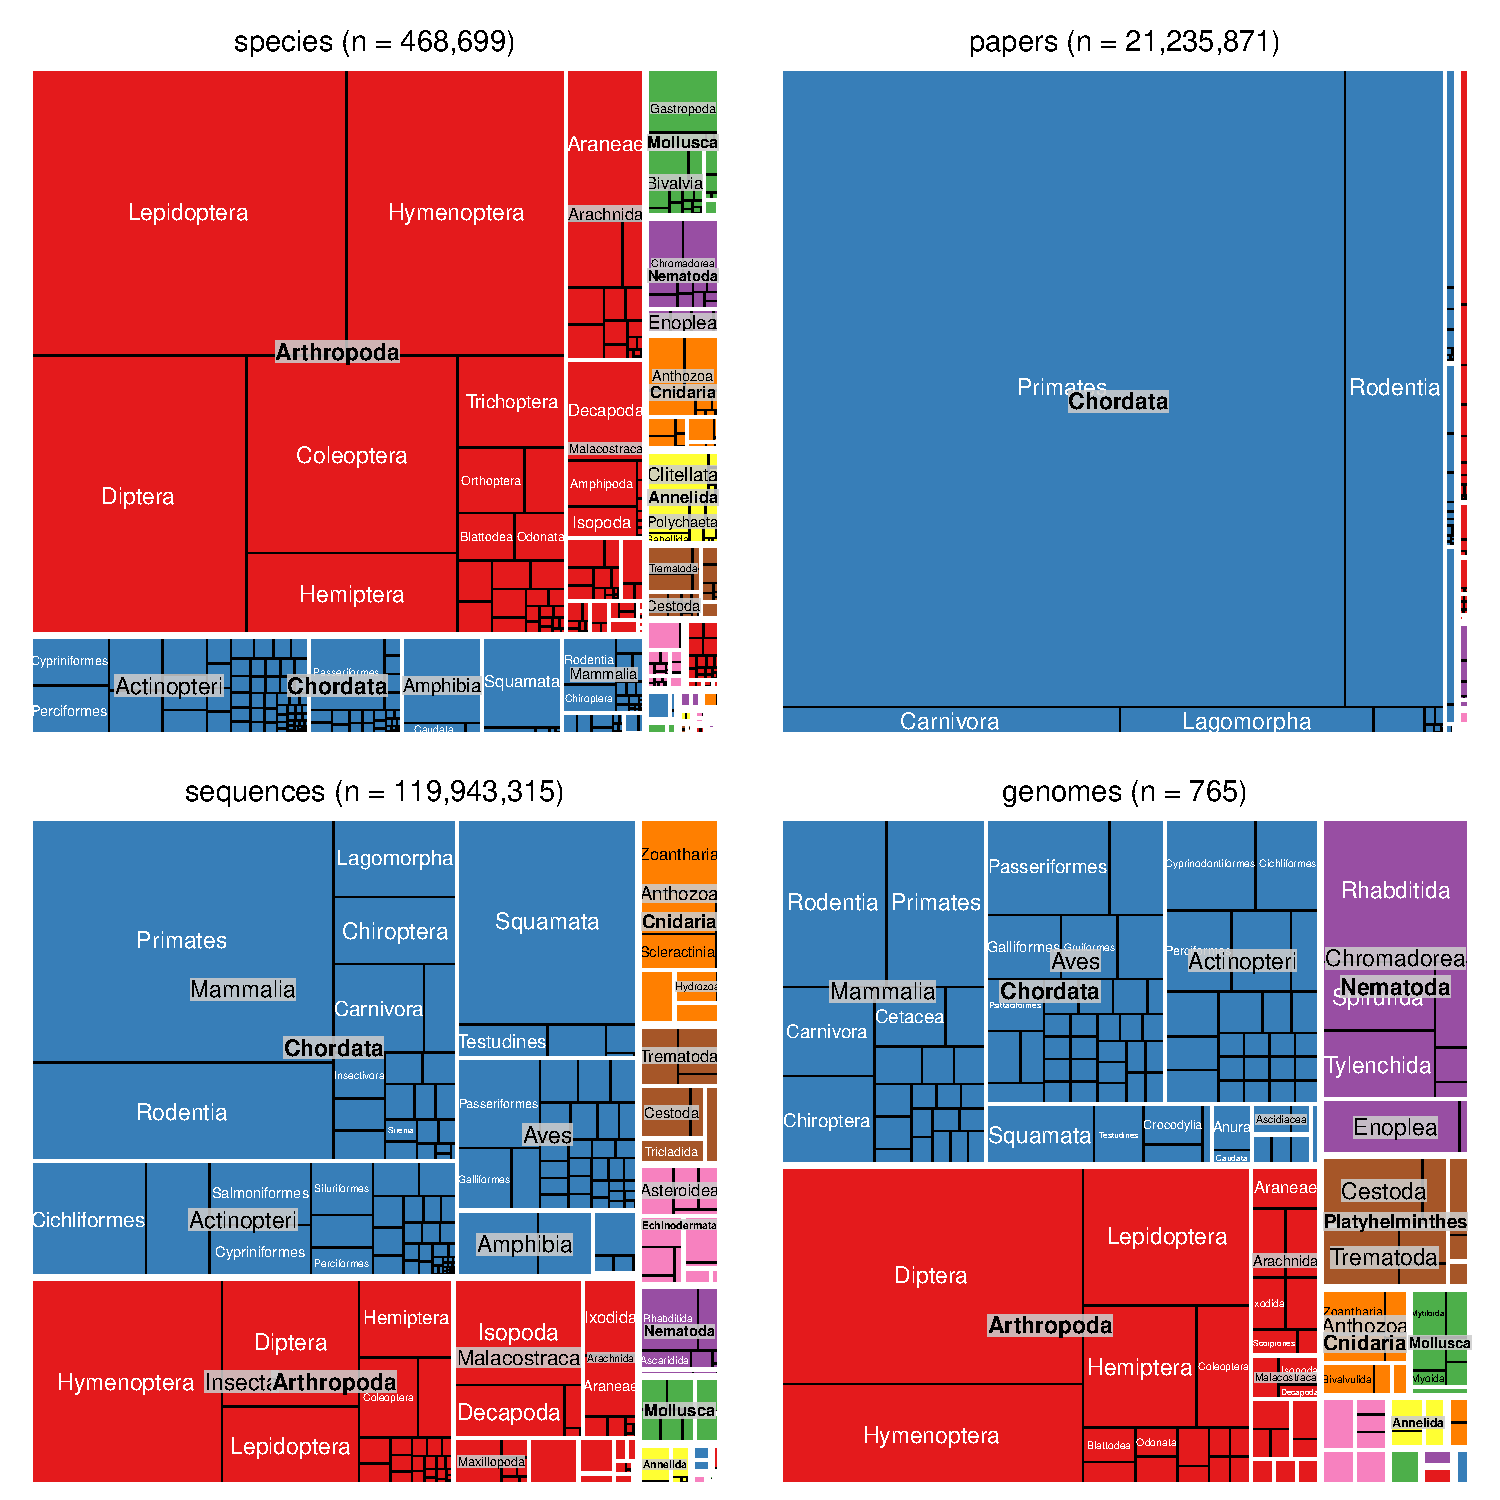
\includegraphics{Fig1}
\caption{Taxonomic diversity of various NCBI databases (considering only
animals). Panels in each plot are scaled to represent the number of database
records corresponding to a given taxonomic rank and are shaded to reflect the
phylum to which they belong. Starting from the upper left in clockwise direction
subplots represent number of species in NCBI Taxonomy, the number of papers 
in PubMed, the number of sequences in NCBI Nucleotide database and the number of 
nuclear genome sequences in NCBI Genome database.}
\label{fig:tm}
\end{center}
\end{figure}

\section{Continued development of \pkg{rentrez}}

\pkg{rentrez} covers the complete EUtils API, is well-documented at the function
and package level and includes an extensive test suite that covers
internal functions as well as typical use-cases of the software. The current
version of \pkg{rentrez} is thus considered a stable release, and it is
unlikely any additional functionality will be added. The software is nevertheless
still actively maintained to keep pace with CRAN and NCBI policies and to fix
any bugs that arise. Software issues, including bug reports and requests for help 
with particular use-cases, are welcomed at the package's software repository:
\url{http://gituhub.com/ropensci/rentrez}.

\section{Acknowledgements}

Development of the \pkg{rentrez} has benefited greatly from being part of the
ROpenSci project. I am especially grateful to Scott Chamberlain for his guidance. 
I am also very grateful to everyone who has provided pull-requests or filed issues 
including Chris Stubben, Karthik Ram, Han Guangchun, Matthew O'Meara, 
Reed Cartwright and Pavel Fedotov.

\bibliography{RJreferences}

\address{David J. Winter\\
  Institute of Fundamental Sciences, Massey University\\
  Palmerston North 4442\\
  New Zealand\\
  ORCiD: 0000-0002-6165-0029 \\
  \email{david.winter@gmail.com}
}

\section{Appendix}

Code used to produce Figure \ref{fig:tm}, using \code{animal\_orders} data generated above.

\begin{example}
    
# Format the total number of records for a graph title
make_title <- function(col_name, data){
    n <- sum(data[,col_name])
    with_commas <- formatC(n, format = "d", big.mark = ",")
    paste0(col_name, " (n = ", with_commas, ")")
}

# Generate a treemap from taxonmic data.frame
# * data= tidy_taxonomy data.frame
# * size_col = name of column for tm tile-size
# * fill_col = name of column for tile-fil
# * row = plot row in 2x2 grid
# * col = plot col in 2x2 grid
# * pal = palette for fill
taxic_diversity_tm <- function(data, size_col, fill_col, row, col, pal){    
    treemap(data, 
        index=c("phylum", "class", "order"), vSize=size_col, vColor=fill_col, 
        palette=pal, type='categorical', position.legend="none", 
        title=make_title(size_col, data), border.col=c("white","white","black"),
        vp = viewport(layout.pos.row = row, layout.pos.col = col)
    )
}

library(treemap)
library(grid)
library(gridExtra)
# 24 phyla means some fill-colours will be re-used, ordering phylum factor by spp
# will prevent any "major" phyla from getting the same colour.
spp_per_phylum <- aggregate(species ~ phylum, FUN=sum, data=animal_orders)
phyla_ordered <- spp_per_phylum$phylum[ order(spp_per_phylum$species, decreasing=TRUE)]
animal_orders$phylum<- factor(animal_orders$phylum, levels=phyla_ordered)
pal <-  rep(RColorBrewer::brewer.pal(8, name="Set1"), 3)

grid.newpage()
pushViewport(viewport(layout = grid.layout(2, 2)))

taxic_diversity_tm(animal_orders, "species",   "phylum", 1,1, pal)
taxic_diversity_tm(animal_orders, "papers",    "phylum", 1,2, pal)
taxic_diversity_tm(animal_orders, "sequences", "phylum", 2,1, pal)
taxic_diversity_tm(animal_orders, "genomes",   "phylum", 2,2, pal)
}
\end{example}
